\documentclass[11pt,twocolumn]{article}
\usepackage{graphicx}
\usepackage[margin=1in]{geometry}
\usepackage{natbib}
\usepackage{amsmath, amssymb, graphicx}
\usepackage{authblk}
\usepackage{url}

\renewcommand\Authfont{\normalsize}
\renewcommand\Affilfont{\small}
\setlength{\affilsep}{0pt}

\providecommand{\apj}{ApJ}
\providecommand{\apjl}{ApJL}
\providecommand{\apjs}{ApJS}
\providecommand{\aap}{A\&A}
\providecommand{\mnras}{MNRAS}
\providecommand{\na}{New Astronomy}
\providecommand{\nat}{Nature}
\providecommand{\jaavso}{JAAVSO}
\providecommand{\aj}{AJ}
\providecommand{\araa}{ARA\&A}
\providecommand{\pasp}{PASP}

\begin{document}

\title{\textbf{The Death of Betelgeuse}}
\author{Brodie Monohan}
\affil{\textit{Whitman College}}
\affil{monohanb@whitman.edu}

\date{December 9, 2025}

\twocolumn[
\begin{@twocolumnfalse}
\maketitle

\begin{abstract}
Betelgeuse has been the focus of extensive observational and theoretical study due to its proximity to Earth and its status as a candidate for the next Galactic type II supernova. Using photometric data from the~\cite{aavso} comprised of 2,924 observations collected by more than 50 observers over the past six decades, I model Betelgeuse's variability as the superposition of a fundamental pulsation period, a long secondary period (LSP), and two overtone periods. These observed periods are then used as constraints in a Zero-Age Main Sequence (ZAMS) stellar evolution model computed with the Modules for Experiments in Stellar Astrophysics (MESA)~\citep{paxton}. By matching the modeled radial pulsation periods to observations and comparing to models from~\citep{saio}, I place Betelgeuse along an evolutionary track and infer its current evolutionary state. I find that Betelgeuse is in a post-giant phase undergoing late-stage core carbon burning, and I estimate that iron core collapse is likely to occur within the next 10 to 430 years.
\end{abstract}

\vspace{1cm}
\end{@twocolumnfalse}
]

\section{Introduction}

\begin{figure*}
    \centering
    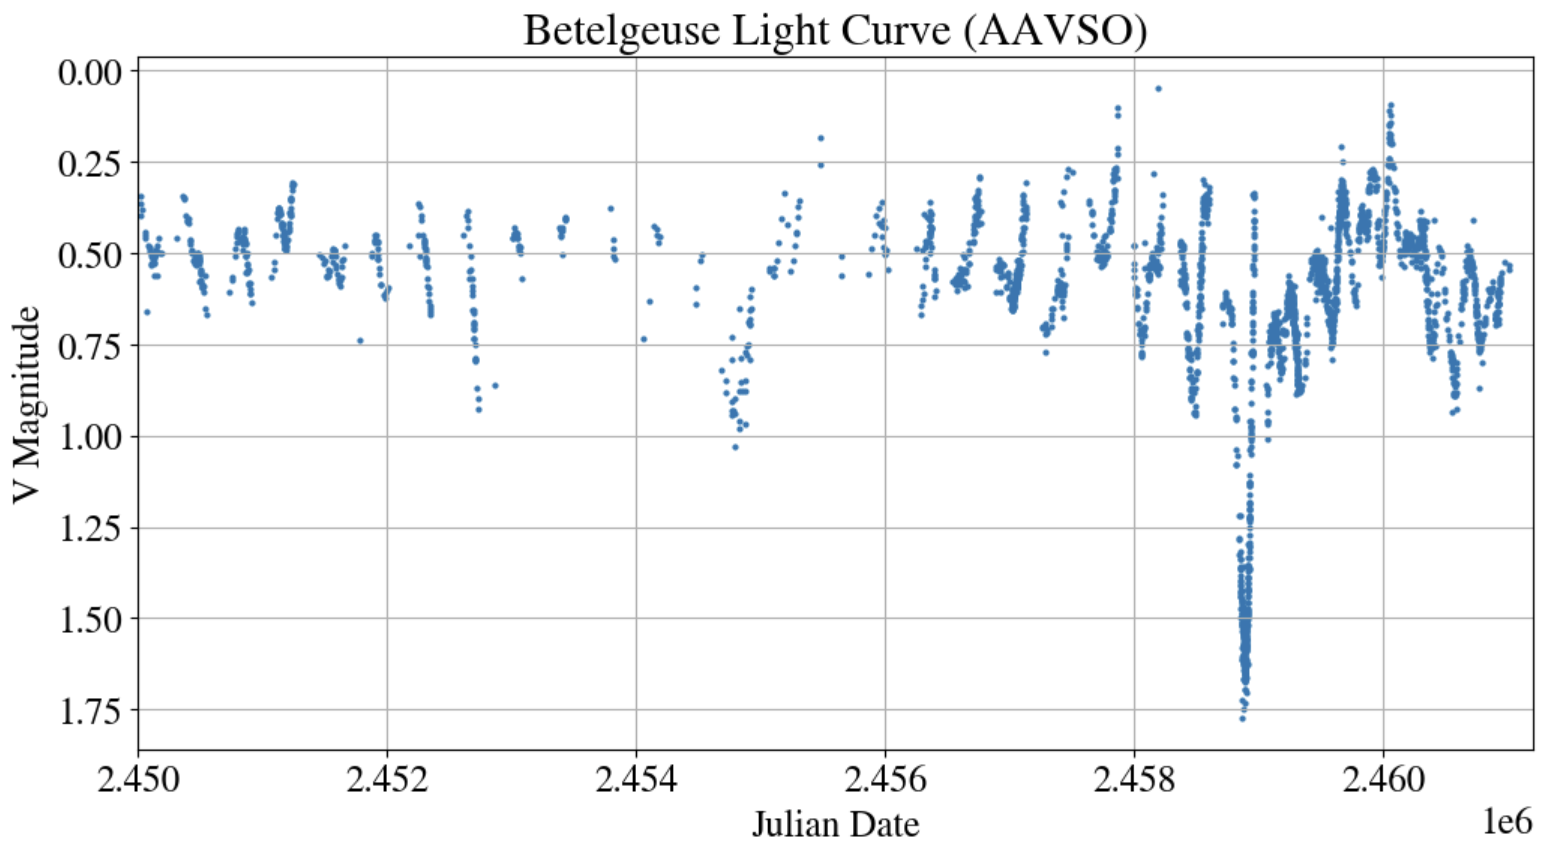
\includegraphics[width=\linewidth]{../figures/lcurve.png}
    \caption{The Betelgeuse light curve over the past $\approx 30$ years from open-source data compiled by AAVSO~\citep{aavso}.}\label{fig:lcurve}
\end{figure*}

For the sun, and main sequence stars in general, nuclear lifetimes are considered ``back of the napkin'' calculations, but this is not the case for an evolved star like Betelgeuse. A nuclear timescale can be found simply by dividing the energy that could be produced by all of the fuel in the core by the amount of energy radiated away per time. This is parameterized by~\citep{pinsonneault} as

\begin{equation}
    t_{\rm nuc}=\frac{E_{\rm core}}{L_\star}=\frac{qM_{\rm core}}{L_\star}
\end{equation}

where $q$ is the energy released per mass of fuel consumed. There are some key factors that make this equation much more complicated, if not impossible practically, to use to describe an evolved stellar lifetime. The most apparent is that we need to know the composition of a star's core and what it is burning. We know from spectroscopy and neutrino detection consistent with the proton-proton chain that the sun is fusing hydrogen, but since Betelgeuse is an evolved star and far away, we cannot do the same precise neutrino detection and spectra won't represent the core because core composition will be very different from surface composition. The second issue is the core mass. With the sun, astronomers have gathered precise helioseismology data which can precisely describe core mass based on longitudinal sound waves. For variable stars, like Betelgeuse, the internal wave structure is much more complicated and obscured by other mechanisms. Because of this, an asteroseismological analysis of the variability of Betelgeuse won't reveal the internal structure in an elementary way like the sun and, as we will see later, only ends up being useful in comprehensive stellar models that account for all the complex internal structure. The third issue is that a simple nuclear timescale formula assumes constant luminosity. In an evolved massive star, $\rm He$ burning, $\rm C$ burning, $\rm Ne$ burning, $\rm O$ burning, and $\rm Si$ burning stages each increase luminosity dramatically. As the core burning stage changes, the rate at which energy is radiated away (our denominator) will change, and again, we do not know what stage Betelgeuse is currently in yet. The last issue is that we must consider the fuel produced in the outer layers of fusion. The available fuel is no longer a single well-defined core mass but a multi-layered, time-dependent structure. In total, a simple nuclear time-scale is not viable to describe the lifetime of an evolved star like Betelgeuse.

\begin{figure*}[t]
    \centering
    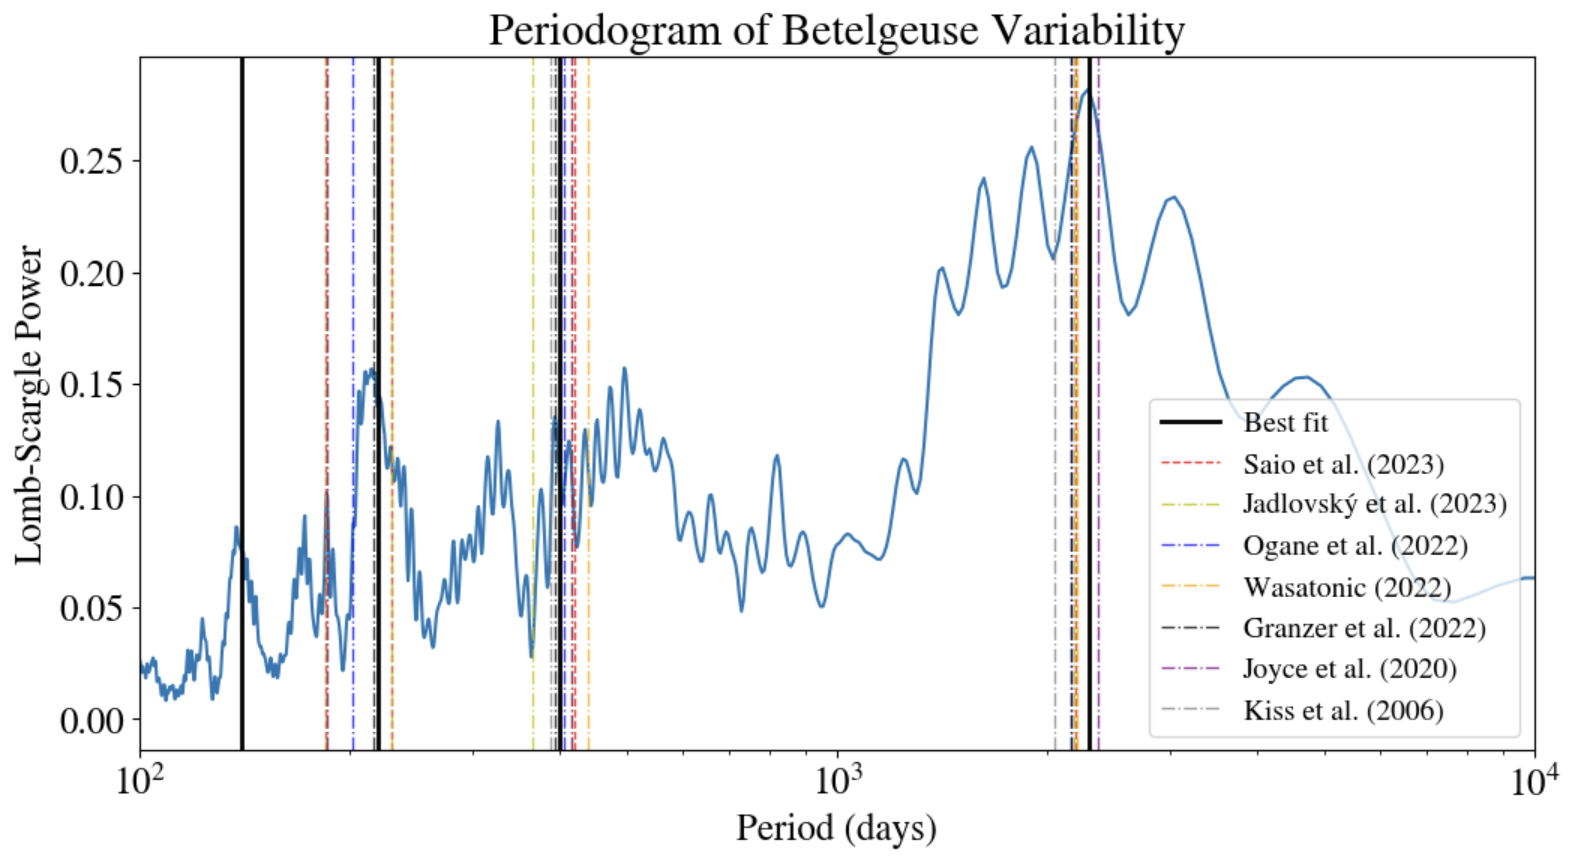
\includegraphics[width=\linewidth]{../figures/periodogram.png}
    \caption{A Lomb-Scargle period analysis of the Betelgeuse light curve showing the Lomb-Scargle power (y-axis) as a function of period in days (x-axis). My best fit for dominant periods in black are 140, 220, 414, and 2293 days in order from left to right. Also plotted are dominant periods identified by~\citep{saio},~\citep{jadlovsky},~\citep{Organe},~\citep{wasatonic},~\citep{granzer},~\citep{joyce}, and~\citep{kiss}.}\label{fig:periodogram}
\end{figure*}

\section{Light Curve Analysis}

A better way to probe Betelgeuse's evolutionary stage is through its variable luminosity. Betelgeuse has a volatile periodic luminosity that indicates radial pulsations caused by $\kappa$ mechanisms (like a Cepheid) which drive and amplify normal modes in the star. These are the target of most attempts to describe the structure, lifetime, and/or evolution of Betelgeuse. There are certain allowed modes within a star called eigen-modes. An eigen-mode is the unique and standing global displacement pattern that a star can sustain without shearing itself apart or the wave canceling itself out with interference. These modes depend on the density profile, the temperature gradient, and the location of the partially ionized zones which excite these modes with $\kappa$ mechanisms, as well as other factors. What matters most is that these modes are fundamental to the structure of the star; what modes are `allowed' (what eigen-modes exist in the star) are directly a product of its composition. Like standing waves on a string, there is a fundamental mode as well as overtone modes ($n=1,2,\ldots$). Unlike standing waves on a string, however, since the density profile is not constant, the overtone modes are not simply half, a third, or some linear combination of a fundamental mode but actually carry information of their own about structure. Because these modes depend on multiple variables and are non-linear, they do not directly translate to a density or temperature profile (at least not that I know of), rather they are most useful when comparing to comprehensive stellar models. The frequency of the corresponding waves that occupy these allowed eigen-modes are called eigen-frequencies. If I can find these eigen-frequencies they will give the best information on the internal structure of Betelgeuse in combination with stellar modeling.

\begin{figure*}
    \centering
    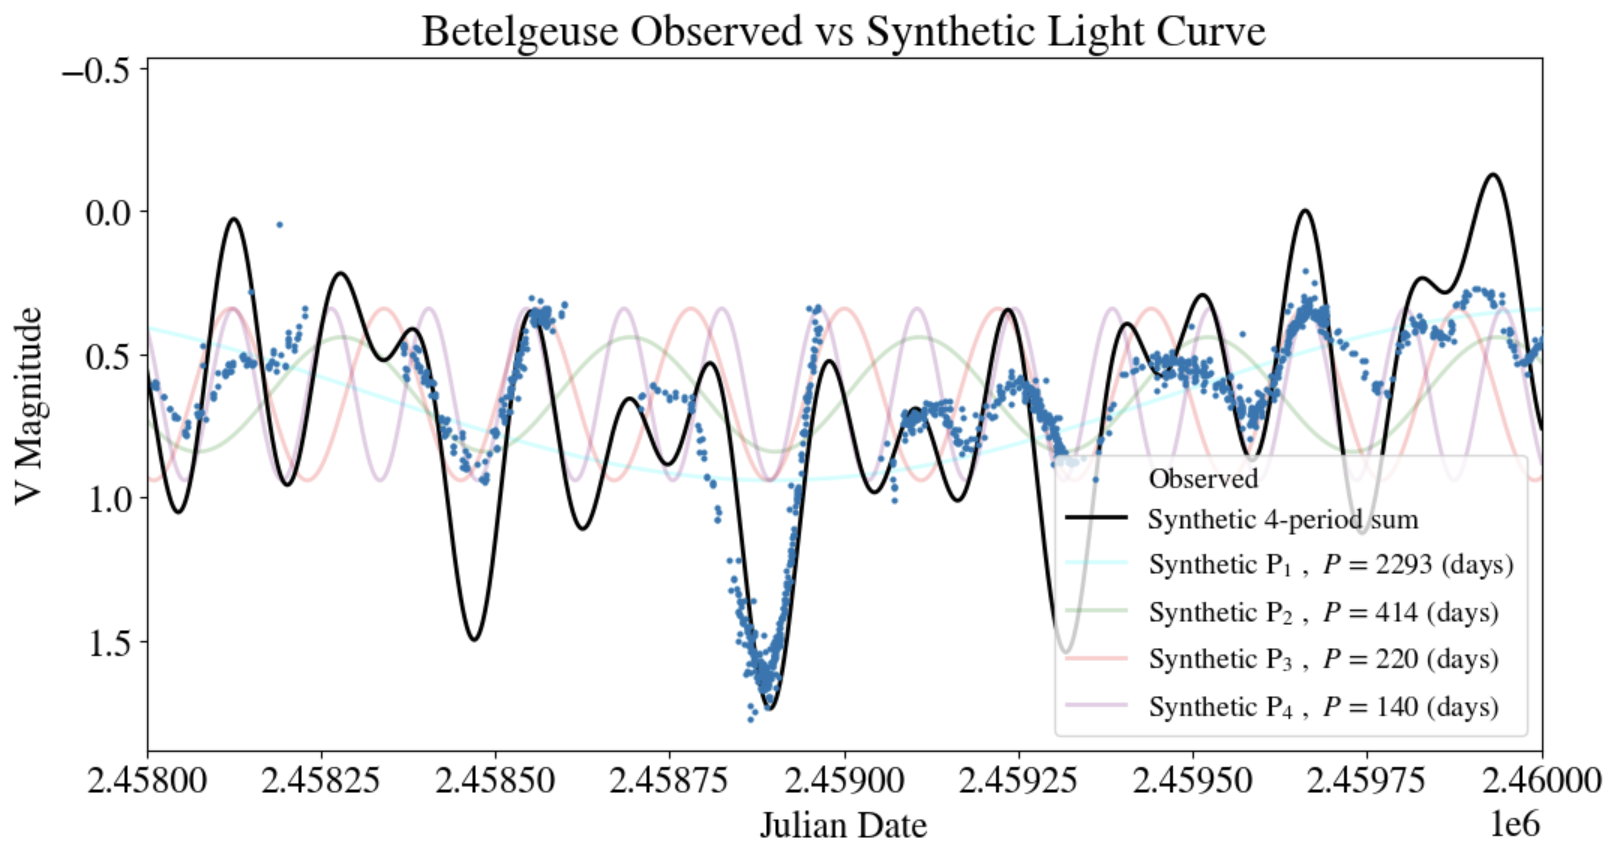
\includegraphics[width=\linewidth]{../figures/lcurve_fit.png}
    \caption{The 4-period synthetic Betelgeuse light curve plotted on top of the observed Betelgeuse light curve near the winter of 2019.}\label{fig:lcurve_fit}
\end{figure*}

To characterize these $\kappa$ mechanism driven eigen-frequencies, I use V-band magnitude data from the American Association of Variable Star Observers (AAVSO) collected from 2,924 observations since 1965, by over 50 different observers~\citep{aavso}. This data shows a clear and complex periodicity in the luminosity of Betelgeuse as seen in Figure 1. Analyzing this luminosity curve with the Lomb-Scargle algorithm, I can pick out the dominant frequencies from a periodogram that shows the Lomb-Scargle power (which measures how well a given period fits a set of data on a scale of 0 to 1) vs period in days. This periodogram and my best-fit for dominant periods are shown in Figure 2. In addition, I include dominant periods chosen by seven other teams studying the periodicity of the Betelgeuse light curve. It is important to note that a period of 2,293 days is almost certainly too long to correspond to an eigen-mode. Of the seven teams plotted, only the~\citep{saio} team considered this period fundamental. Others call this feature the Long Secondary Period (LSP) and suggest it could be a convective feature, periodically bringing energy from deeper in the star to the surface that happens to have a steady frequency in larger red giant stars. From these chosen fundamental frequencies and a LSP, I superimposed them together to create a synthetic light curve which I fit to the actual Betelgeuse light curve as seen in Figure 3. Amplitude and phase were chosen by eye to best fit the overall shape of the light curve near the winter of 2019, called `the great darkening'. This event, where Betelgeuse's luminosity dropped to its lowest point in its over 60 year recorded history, is almost certainly the product of negative constructive interference in these dominant periods and serves as a good phasal anchor point.

\section{Modeling}
To model a variable star like Betelgeuse and its radial pulsations I first need to decide is if they should be modeled adiabatically or non-adiabatically. To do this I can compare the fundamental period to the thermal time of the star. If the fundamental pulsation period is short compared to the thermal time then heat transfer between layers can be estimated as 0 (the initial condition and final condition are indistinguishable over a single pulse). This adiabatic condition looks like
\begin{equation}
    t_{\rm th}=\frac{1}{2}t_{\rm KH}=-\frac{U_\star}{2L_\star} \gg \rm P_0
\end{equation}


as described by~\citep{pinsonneault}. The thermal time depends on the mass, which is unknown at this point, but if the fundamental period is 414 or 2,293 days, this certainly won't hold for a range of masses feasible for Betelgeuse. Cepheids typically have periods on the order of days to months and start to be described better non-adiabatically with periods over about a week. None of my chosen periods will be model-able adiabatically even though Betelgeuse presumably has a relatively high mass.

With a synthetic light curve composed of a superposition of 3 fundamental eigen-mode periods and a LSP, I can build a comprehensive stellar model to match these periods. This will fit Betelgeuse to an evolutionary track, fusion stage, and remaining lifetime, as well constrain and estimate other features like radius, mass, and temperature. To do this I would use MESA to generate stellar models and its extension for asteroseismolocial analysis, GYRE, to analyze the produced light curves. However, this requires knowledge and time (and potentially a super-computer) that are out of the scope of this project. Instead, I use the Zero Age Main Sequence (ZAMS) parameters generated by the~\citep{saio} team, whose chosen periods most closely matched mine, in conjunction with the Mad Star MESA-web program hosted by the University of Wisconsin \citep{madstar}. The parameters I adopted were ${ M_{\rm ZAMS}} = {\rm 19M_\odot} $, $X=0.709$, $Z=0.020$, $\Omega_{\rm ZAMS}/\Omega_{\rm crit}=0.2$, and $\rm{MLA}=1.6$.

\section{Results}

The~\citep{saio} team found a current luminosity of $\log(L/L_\odot)=5.27$ and current effective temperature of $\log(T_{\rm eff})=3.52 {\rm K}$ in late-stage carbon burning based on their models. In late-stage carbon burning, my model produces a similar luminosity near $\log(L/L_\odot) \approx 5.2$ and an effective temperature about 0.5 orders of magnitude too high at $\log(T_{\rm eff})\approx 4.1 {\rm K}$. This means my model lifetime may be skewed slightly shorter as more heat will cause fusion stages to initiate earlier than they otherwise would but this is only an effective temperature and does not give information on the temperature gradient or the temperature of the core in either model so the actual effects of this effective temperature discrepancy are unknown.
\begin{figure}
    \centering
    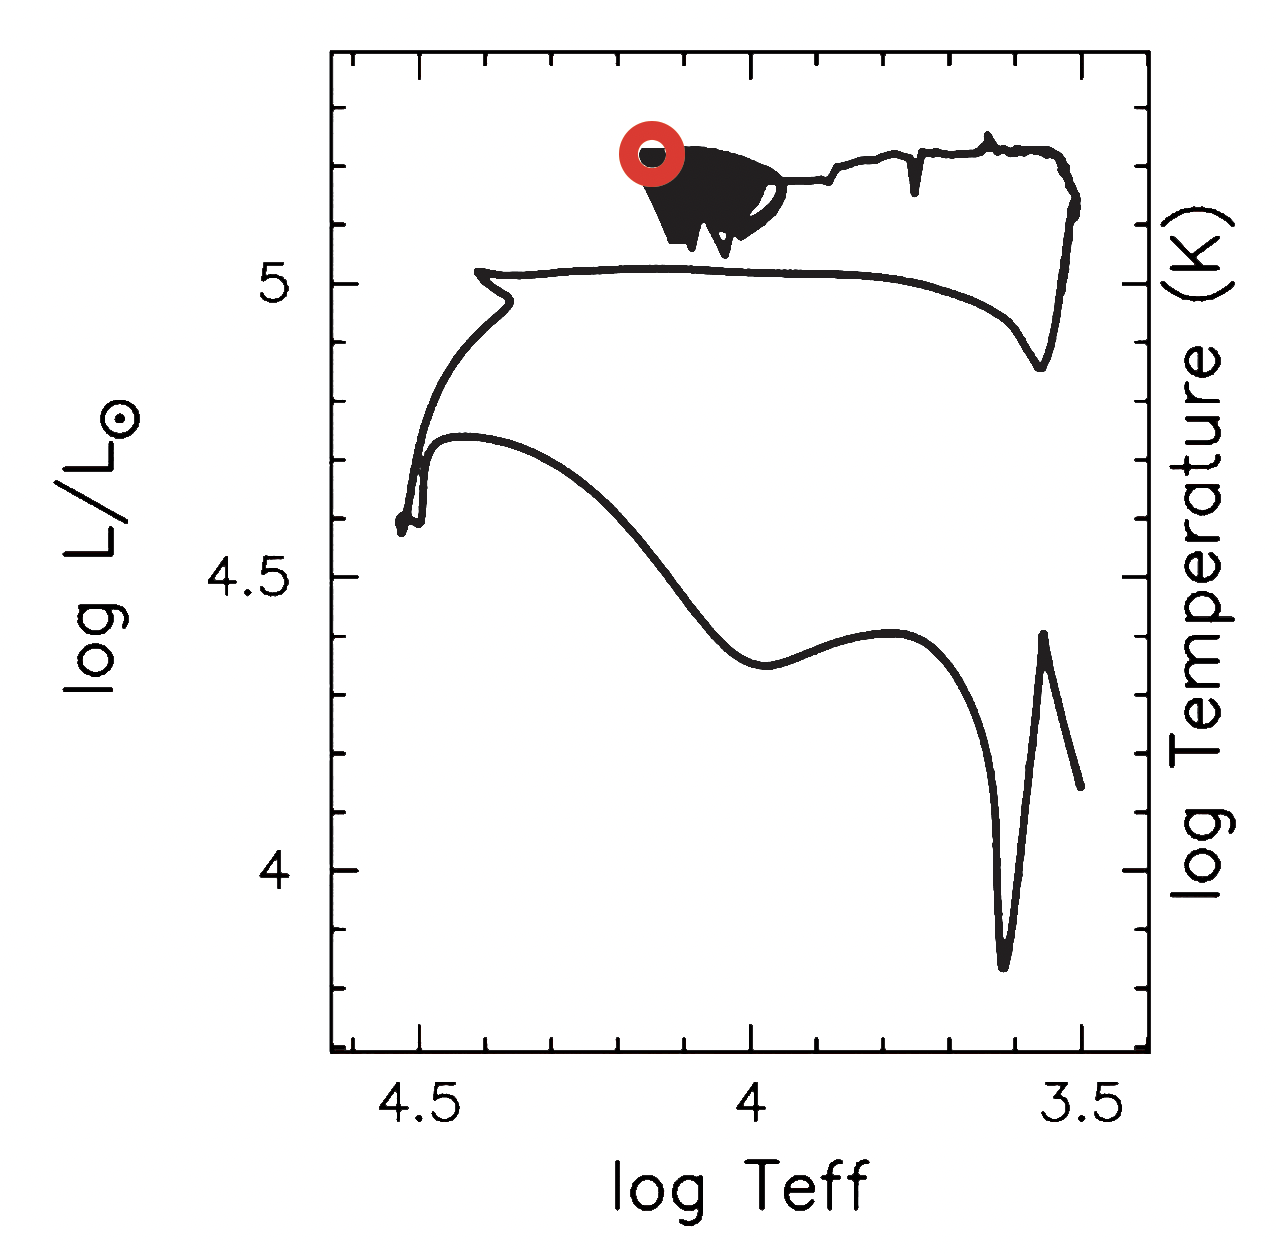
\includegraphics[width=\linewidth]{../figures/mesa.png}
    \caption{The position of late stage carbon burning for the model Betelgeuse on a luminosity-temperature Hertzsprung-Russel diagram.}\label{fig:mesa}
\end{figure}

\section{Conclusion}

I find 4 dominant frequencies in the Betelgeuse light curve using Lomb-Scargle analysis, 3 of which correspond to eigen-frequencies that are fundamental to the structure of the star. With these periods I create a model based on ZAMS parameters of models that produce similar fundamental $\kappa$ mechanism periods from~\citep{saio}. Assuming Betelgeuse is in a late carbon burning stage, my model predicts a remaining lifetime of 10 to 430 years before iron core collapse.

\bibliographystyle{apalike}
\bibliography{ref}

\end{document}